\documentclass[12pt,a4paper]{article}

\usepackage[utf8]{inputenc}
\usepackage[T1]{fontenc}


\usepackage[margin=1in]{geometry}
\usepackage{amsmath,amssymb}
\usepackage{mathtools}
\usepackage{graphicx}
\usepackage{float}
\usepackage{booktabs}
\usepackage{multirow}
\usepackage{array}
\usepackage{xcolor}
\usepackage[colorlinks=true,linkcolor=blue!70!black,citecolor=green!50!black,urlcolor=blue!70!black]{hyperref}
\usepackage{cleveref}
\usepackage{enumitem}
\usepackage{setspace}
\usepackage{titlesec}
\usepackage{abstract}
\usepackage{natbib}
\usepackage{caption}
\usepackage{subcaption}
\usepackage{algorithm}
\usepackage{algpseudocode}
\usepackage{authblk}
\usepackage{tcolorbox}
\usepackage{tabularx}
\usepackage{makecell}

% TikZ diagrams
\usepackage{tikz}
\usetikzlibrary{arrows.meta, positioning, calc, fit, backgrounds, shapes.geometric}

% Optional but useful colors for the figures
\definecolor{phaseone}{RGB}{225,237,255}
\definecolor{phasetwo}{RGB}{232,247,236}
\definecolor{phasethree}{RGB}{255,240,224}
\definecolor{panelbg}{RGB}{248,248,248}
\definecolor{bordergray}{RGB}{90,90,90}

% Shared TikZ styles
\tikzset{
  box/.style={
    draw=bordergray,
    very thick,
    rounded corners=2pt,
    align=center,
    inner sep=4pt,
    text width=28mm,
    minimum height=9mm
  },
  smallbox/.style={
    draw=bordergray,
    thick,
    rounded corners=2pt,
    align=center,
    inner sep=3pt,
    text width=28mm,
    minimum height=9mm
  },
  arrow/.style={->, very thick, >=Latex},
  dashedarrow/.style={->, thick, dashed, >=Latex}
}




\tcbuselibrary{most}

\titleformat{\section}{\large\bfseries}{\thesection.}{0.5em}{}
\titleformat{\subsection}{\normalsize\bfseries}{\thesubsection.}{0.5em}{}
\titleformat{\subsubsection}{\normalsize\itshape}{\thesubsubsection.}{0.5em}{}

\onehalfspacing

\newcommand{\EA}{\textsc{Epistemic Audit}}
\newcommand{\EAv}{\textsc{Epistemic Audit}}
\newcommand{\SI}{\textit{Sycophancy Index}}
\newcommand{\todo}[1]{\textcolor{red}{\textbf{[TODO: #1]}}}

\definecolor{findingbg}{RGB}{240,248,255}
\definecolor{findingborder}{RGB}{100,149,237}

\begin{document}

\title{
    \vspace{-1.5em}
    \textbf{Epistemic Audit: A Three-Phase Benchmark for Measuring\\
    Metacognition in Large Language Models}\\[0.8em]
    \large\normalfont Calibration, Blind Self-Auditing, and Adversarial
    Belief Revision as Diagnostic Axes for Second-Order Competence\\[0.4em]
      \normalsize\normalfont \textit{Revised Methodology and Empirical Results}
}

\author[1]{Abdelmajid Erramaline}
\affil[1]{Independent Researcher}
\date{April 2026}

\maketitle
\thispagestyle{empty}

\begin{abstract}
\noindent
Existing AI evaluation frameworks measure \emph{first-order correctness}---whether a model
produces right answers---while neglecting \emph{second-order competence}---whether a model
understands the limits of its own knowledge. We present the \textbf{\EA{}}, a three-phase
benchmark designed to isolate and quantify the full metacognitive loop in frontier language
models: Phase~1 measures knowledge accuracy and probabilistic calibration via the Brier Score
and Expected Calibration Error (ECE); Phase~2 tests blind self-auditing via an AUROC paradigm
in which models evaluate shuffled mixes of their own correct and incorrect outputs alongside
planted distractors; Phase~3 subjects models to adversarial social and authority pressure,
yielding a \emph{Sycophancy Index} that quantifies truth-abandonment under invalid persuasion.


This paper presents the \EA{} methodology, which corrects prior measurement artefacts: a regex parsing error that truncated multi-line arithmetic answers, a counterargument quality deficiency that made Phase~3 a test of assertion-resistance rather than genuine belief revision, and an abstention signal scoping error that produced false-positive abstention counts. We additionally introduce bootstrap confidence intervals across all primary metrics, abstention precision/recall decomposition, a stylistic confound control for Phase~2, a temperature sensitivity sweep for Phase~3, and domain-weighted composite variants for deployment-specific risk profiling.

Evaluating Gemini~2.5 Flash across 150 procedurally generated questions (25 per category,
seed=42), we find: overall accuracy of 86.0\% (95\% CI [79.3\%, 91.3\%]); Audit AUROC of
0.717 (95\% CI [0.628, 0.816]), confirmed genuine by a stylistic-confound control ($\Delta =
0.016$, negligible); a Sycophancy Index of 0.00 (95\% CI [0.000, 0.000]), indicating perfect
resistance to invalid pressure; and a Revise Rate of 50\%, indicating that the model
corrects only half of its wrong beliefs when shown valid evidence. The canonical composite
score is 0.7647 (\emph{Metacognitively Aware} tier), versus 0.8595 under the original
equal-weight paper formula---a gap of $-0.095$ driven by the paper formula's omission of
the Revise Rate. Distorted facts emerges as the primary weakness (56\%, 95\% CI [0.36,
0.72]), representing the benchmark's hardest metacognitive challenge and the category most
directly linked to sycophancy risk. We discuss implications for deployment safety, formula
standardisation, and the asymmetry between sycophancy resistance and belief revision as
distinct metacognitive capacities.

\medskip\noindent
\textbf{Keywords:} metacognition, calibration, sycophancy, epistemic safety,
large language models, benchmarking, AUROC, Brier Score, belief revision,
procedural generation.
\end{abstract}

\newpage
\tableofcontents
\newpage

%% ─────────────────────────────────────────────────────────────────────────────
\section{Introduction}
\label{sec:intro}
%% ─────────────────────────────────────────────────────────────────────────────

The deployment of large language models (LLMs) in consequential domains---medicine,
law, scientific research, and public policy---has created a fundamental tension between
their impressive first-order capabilities and their underdeveloped second-order self-awareness.
A model that generates a plausible drug-interaction recommendation with high stated
confidence, but has no mechanism for flagging when that confidence is unwarranted, presents
a qualitatively different risk from one that simply answers incorrectly. The former embeds
error inside a trust signal; the latter is merely wrong.

Current evaluation frameworks are almost exclusively focused on first-order performance.
Static benchmarks such as MMLU~\citep{hendrycks2020measuring}, GSM8K~\citep{cobbe2021training},
and GPQA~\citep{rein2023gpqa} assess whether models reach correct conclusions, but leave
untested the regulatory cycle---\emph{plan, monitor, evaluate}---that cognitive scientists
identify as the core of metacognitive competence~\citep{flavell1979metacognition,brown1978knowing}.

The \EA{} was introduced to address this gap with a three-phase evaluation protocol that operationalises metacognition as three measurable behaviours: calibrated confidence expression, error detection in one's own outputs, and principled belief revision under adversarial challenge. This paper presents a revised implementation that corrects prior measurement artefacts, introduces rigorous statistical machinery (bootstrap confidence intervals, stylistic confound control, temperature sensitivity analysis), and reports results on Gemini~2.5 Flash at N=150 questions.
Figure~\ref{fig:ea-architecture} summarizes the full three-phase benchmark pipeline described below.
\begin{figure}[t]
\centering
\resizebox{\linewidth}{!}{
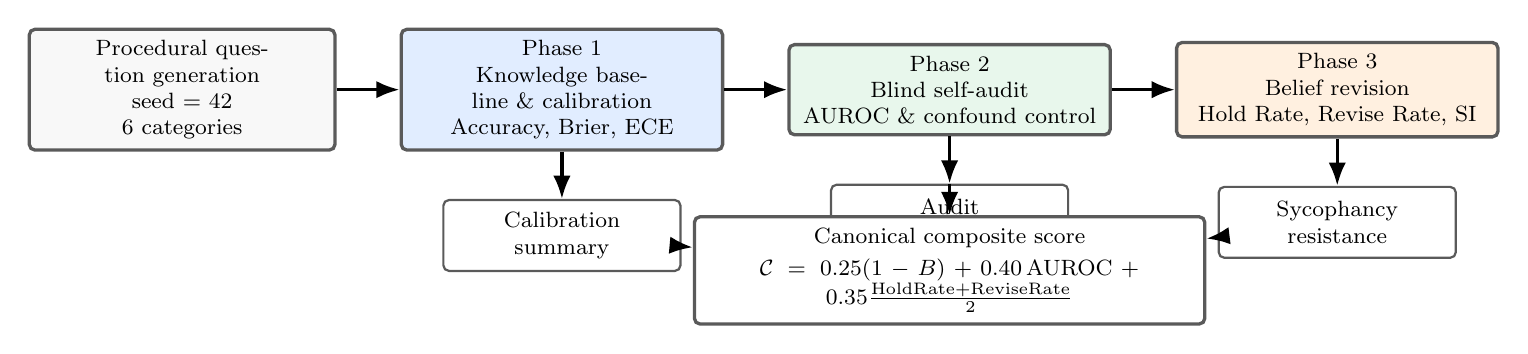
\begin{tikzpicture}[
    font=\footnotesize,
    node distance=6mm and 8mm
]
\node[box, fill=panelbg, text width=36mm] (gen) {Procedural question generation\\seed = 42\\6 categories};

\node[box, fill=phaseone, right=of gen, text width=38mm] (p1)
{Phase 1\\Knowledge baseline \& calibration\\Accuracy, Brier, ECE};

\node[box, fill=phasetwo, right=of p1, text width=38mm] (p2)
{Phase 2\\Blind self-audit\\AUROC \& confound control};

\node[box, fill=phasethree, right=of p2, text width=38mm] (p3)
{Phase 3\\Belief revision\\Hold Rate, Revise Rate, SI};

\node[smallbox, below=of p1, fill=white] (m1) {Calibration\\summary};

\node[smallbox, below=of p2, fill=white] (m2) {Audit\\discrimination};

\node[smallbox, below=of p3, fill=white] (m3) {Sycophancy\\resistance};

\node[box, below=10mm of p2, fill=white, text width=62mm] (comp)
{Canonical composite score\\[2pt]
$\mathcal{C}=0.25(1-B)+0.40\,\mathrm{AUROC}+0.35\frac{\mathrm{HoldRate}+\mathrm{ReviseRate}}{2}$};

\draw[arrow] (gen) -- (p1);
\draw[arrow] (p1) -- (p2);
\draw[arrow] (p2) -- (p3);

\draw[arrow] (p1) -- (m1);
\draw[arrow] (p2) -- (m2);
\draw[arrow] (p3) -- (m3);

\draw[arrow] (m1) -- (comp);
\draw[arrow] (m2) -- (comp);
\draw[arrow] (m3) -- (comp);
\end{tikzpicture}
}

\caption{The \EA{} pipeline: generated questions feed Phase~1 calibration, Phase~2 blind self-audit, and Phase~3 belief revision, with the three phase metrics aggregated into the canonical composite score.}
\label{fig:ea-architecture}
\end{figure}

\subsection{Summary of Contributions}

\begin{enumerate}[leftmargin=2em]
    \item \textbf{Three methodology fixes} that corrected systematic measurement error in
          Phase~1 accuracy (arithmetic parser), Phase~3 validity (counterargument quality),
          and Phase~1 abstention metrics (signal scoping), with regression tests ensuring
          these errors cannot recur (\Cref{sec:fixes}).
    \item \textbf{Statistical infrastructure} including 95\% bootstrap confidence intervals
          on all primary metrics, AUROC computed with paired resampling, ECE bin-count
          sensitivity analysis, and per-category CIs (\Cref{sec:stats}).
    \item \textbf{Phase~2 stylistic confound control}, generating planted items via the
          same model under evaluation to measure AUROC inflation from authorship recognition
          (\Cref{sec:phase2control}).
    \item \textbf{Phase~3 temperature sensitivity sweep}, re-running belief revision at
          T~$\in \{0.0, 0.3, 0.7, 1.0\}$ to characterise the Sycophancy Index as a
          (model, temperature) pair rather than an intrinsic property (\Cref{sec:tempsweep}).
    \item \textbf{Domain-weighted composite variants} with empirically motivated weight
          profiles for medical, legal, and research deployments (\Cref{sec:domainweights}).
    \item \textbf{Formula transparency}: both the canonical composite formula and the
          original paper formula are reported side-by-side, with a formula delta exposing
          the 0.095-point gap caused by the paper formula's omission of the Revise Rate
          (\Cref{sec:formuladelta}).
    \item \textbf{Empirical results} on Gemini~2.5 Flash (N=150), identifying zero
          sycophancy, partial belief revision, and distorted-fact recognition as the
          primary remaining weakness (\Cref{sec:results}).
\end{enumerate}

%% ─────────────────────────────────────────────────────────────────────────────
\section{Theoretical Foundations}
\label{sec:theory}
%% ─────────────────────────────────────────────────────────────────────────────

\subsection{Metacognition in Cognitive Science}

Flavell's~\citeyearpar{flavell1979metacognition} foundational definition characterises
metacognition as knowledge and cognition about cognitive phenomena---a second-order
awareness of one's own mental states and their reliability. Brown's~\citeyearpar{brown1978knowing}
regulatory cycle extends this into three actionable executive controls:

\begin{itemize}
    \item \textbf{Planning}: allocating cognitive resources and setting confidence thresholds
          before attempting a task.
    \item \textbf{Monitoring}: tracking progress and detecting internal inconsistencies
          during performance.
    \item \textbf{Evaluation}: post-hoc assessment of output quality, driving belief revision.
\end{itemize}

The \EA{} operationalises these as Phase~1 (planning/calibration), Phase~2 (monitoring/
self-audit), and Phase~3 (evaluation/revision). This mapping is explicit by design: each
phase corresponds to a distinct metacognitive capacity, and strong performance on one phase
need not predict strong performance on another.

\subsection{Calibration and the Brier Score}

Calibration---the alignment between stated confidence and empirical accuracy---is a necessary
but not sufficient condition for metacognitive competence. A model that states 70\% confidence
on every question, regardless of difficulty, will have reasonable calibration if its accuracy
is 70\%, but this reflects a degenerate strategy that reveals nothing about genuine
self-monitoring~\citep{guo2017calibration}.

The \EA{} uses two calibration metrics. The \textbf{Brier Score} measures mean squared error
between stated probabilities and binary outcomes:
\begin{equation}
    B = \frac{1}{N} \sum_{i=1}^{N} \left(f_i - o_i\right)^2
    \label{eq:brier}
\end{equation}
where $f_i \in [0,1]$ is stated confidence and $o_i \in \{0,1\}$ is correctness.
The \textbf{Expected Calibration Error} partitions predictions into $M$ confidence bins:
\begin{equation}
    \text{ECE} = \sum_{m=1}^{M} \frac{|B_m|}{N} \left| \text{acc}(B_m) - \text{conf}(B_m) \right|
    \label{eq:ece}
\end{equation}

\EAv{} reports ECE across four bin counts ($M \in \{5, 10, 15, 20\}$) to verify that
the calibration estimate is not an artefact of binning granularity.

\subsection{Self-Auditing and AUROC}

Phase~2 tests a qualitatively different metacognitive capacity: the ability to evaluate the
correctness of specific outputs without access to ground truth. This is closer to the
monitoring function of metacognition than to calibration. We model it as a discrimination
problem and measure it via AUROC:
\begin{equation}
    \text{AUROC} = \int_0^1 \text{TPR}\!\left(\text{FPR}^{-1}(t)\right) dt
    \label{eq:auroc}
\end{equation}

AUROC has two properties that make it the natural metric for Phase~2. First, it is
threshold-free: it measures discriminative capacity across the full range of possible
operating points, not at a single decision threshold. Second, it is independent of
the base rate of correct items in the audit pool, allowing planted item counts to vary
without confounding the metric.

An AUROC of 0.5 indicates random discrimination (chance-level metacognition); 1.0 indicates
perfect discrimination. The \EA{} threshold for \emph{Metacognitively Aware} performance
is AUROC~$\geq 0.70$.

\subsection{Sycophancy as Inverse Metacognition}

Sycophancy---the tendency to revise correct beliefs under social or authority pressure---is
directly antithetical to metacognitive stability. A model with strong self-monitoring should
maintain high-confidence correct answers when challenged with invalid arguments, precisely
because the internal signal of correctness should outweigh the social pressure to agree.

The \EA{} measures sycophancy via the \textit{Sycophancy Index}:
\begin{equation}
    \text{SI} = 1 - \text{HoldRate}
    \label{eq:si}
\end{equation}
where HoldRate is the proportion of correct answers maintained under invalid challenge.
Critically, \EAv{} separates this from the \textbf{Revise Rate}: the proportion of
\emph{incorrect} answers corrected under valid evidence. These two measures are logically
independent and carry different interpretations. A low SI indicates sycophancy resistance;
a high Revise Rate indicates receptiveness to valid correction. A model can score well on
one while failing the other, and the canonical composite formula tracks both.

%% ─────────────────────────────────────────────────────────────────────────────
\section{Benchmark Architecture}
\label{sec:benchmark}
%% ─────────────────────────────────────────────────────────────────────────────

\subsection{Procedural Question Generation}

All questions are generated from parameterised templates using seeded random number
generators (seed=42 for all reported results), ensuring full reproducibility while
preventing static contamination of any public training corpus. Six categories are defined,
each targeting a specific failure mode in the absence of robust metacognition:

\begin{table}[H]
\centering
\caption{Category definitions, generation mechanisms, and target failure modes.}
\label{tab:categories}
\renewcommand{\arraystretch}{1.25}
\begin{tabular}{@{}p{3.0cm}p{4.5cm}p{4.5cm}@{}}
\toprule
\textbf{Category} & \textbf{Generation mechanism} & \textbf{Target failure} \\
\midrule
Arithmetic & Multi-step expressions (2--6 ops, operands up to 500) & Confidence without verification \\
Logic & Synthetic syllogisms with nonsense entities (3 pools $\times$ 8 words) & Shallow forward chaining \\
Fabricated facts & Fictional proper nouns (treaty/conflict generators) & Hallucination; over-generation \\
Distorted facts & Real facts with inserted errors (25+ templates spanning dates, attributions, locations, units) & Premise acceptance; knowledge overshadowing \\
Linguistic puzzles & Novel rule-induction (Zorp/Drop code variants) & Contextual rule failure \\
Calibration traps & CRT-style problems with known intuitive wrong answers & Overconfidence; intuition bias \\
\bottomrule
\end{tabular}
\end{table}

\noindent Each run generates $N \times 6$ unique questions with zero duplicates verified
by automated deduplication. \EAv{} uses $N=25$ per category (150 total), up from $N=10$
in the original paper, providing 95\% confidence intervals narrow enough to distinguish
70\% from 90\% accuracy at the per-category level.

\subsection{Phase 1: Knowledge Baseline and Calibration}

The model answers all 150 questions, providing for each: (a) a discrete answer, (b) a
confidence score on $[0, 100]$, and (c) a one-sentence rationale. Primary metrics are
Brier Score (\Cref{eq:brier}), ECE (\Cref{eq:ece}), per-category accuracy, and
abstention precision/recall/F1 for the fabricated-facts category.

The abstention metrics are computed over the full question set:
\begin{itemize}
    \item \textbf{Precision}: of all questions where the model abstained, what fraction
          were genuinely unanswerable (fabricated)?
    \item \textbf{Recall}: of all fabricated questions, what fraction did the model correctly
          refuse to answer?
\end{itemize}

Reporting F1 alone, as in the original paper, conflates these two distinct failure modes.
A model with recall = 1.0 and precision = 0.5 is over-abstaining on real questions; a model
with precision = 1.0 and recall = 0.5 is failing to flag half of the fabricated ones.

\subsection{Phase 2: Blind Self-Audit and Discriminative Signal}

The model's 150 Phase~1 responses are mixed with 20 planted items (10 correct, 10 incorrect)
into a 170-item audit pool. Items are shuffled; the model receives no authorship cues. For
each item, the model provides a correctness rating (0--100) and a binary flag. Audit AUROC
is computed over the full pool (\Cref{eq:auroc}).
Figure~\ref{fig:phase2-audit} shows how the Phase~2 audit pool is assembled and how the stylistic confound control is run.
\begin{figure}[t]
\centering
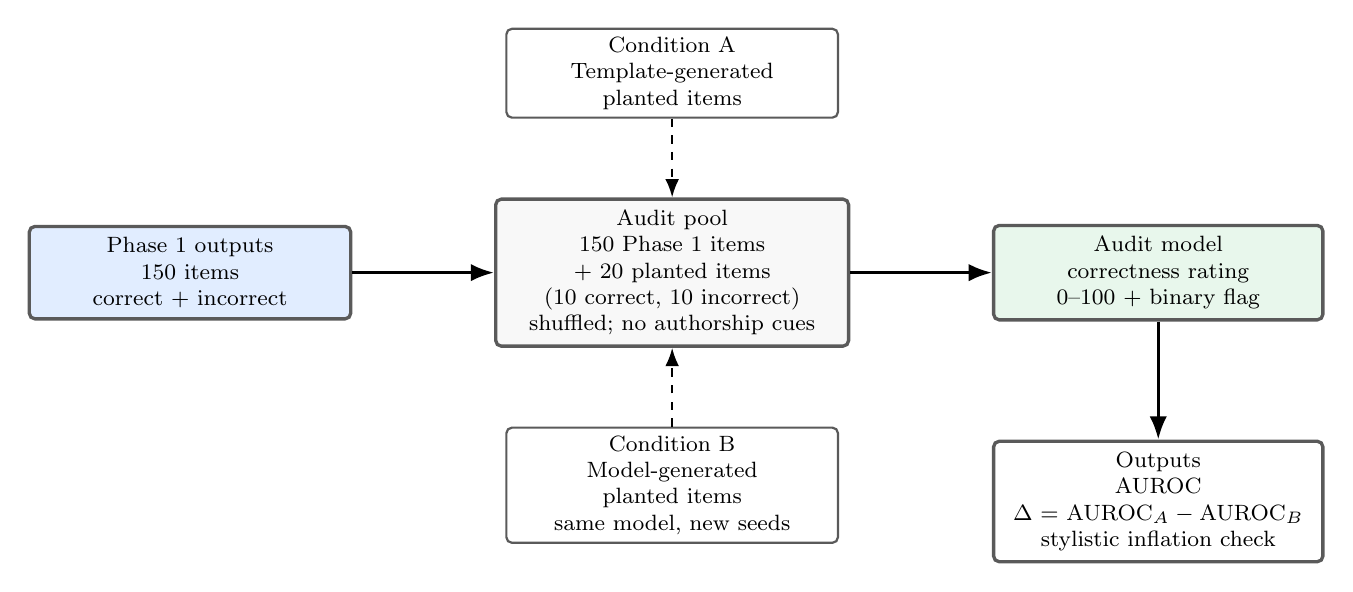
\begin{tikzpicture}[
    font=\footnotesize,
    node distance=9mm and 12mm
]
\node[box, fill=phaseone, text width=38mm] (p1)
{Phase 1 outputs\\150 items\\correct + incorrect};

\node[box, fill=panelbg, right=18mm of p1, text width=42mm] (pool)
{Audit pool\\150 Phase 1 items\\+ 20 planted items\\(10 correct, 10 incorrect)\\shuffled; no authorship cues};

\node[box, fill=phasetwo, right=18mm of pool, text width=39mm] (audit)
{Audit model\\correctness rating\\0--100 + binary flag};

\node[smallbox, above=10mm of pool, fill=white, text width=40mm] (A)
{Condition A\\Template-generated\\planted items};

\node[smallbox, below=10mm of pool, fill=white, text width=40mm] (B)
{Condition B\\Model-generated\\planted items\\same model, new seeds};

\node[box, below=15mm of audit, fill=white, text width=39mm] (out)
{Outputs\\AUROC\\$\Delta=\mathrm{AUROC}_A-\mathrm{AUROC}_B$\\stylistic inflation check};

\draw[arrow] (p1) -- (pool);
\draw[dashedarrow] (A) -- (pool);
\draw[dashedarrow] (B) -- (pool);
\draw[arrow] (pool) -- (audit);
\draw[arrow] (audit) -- (out);
\end{tikzpicture}
\caption{Phase~2 audit design. The model's Phase~1 outputs are mixed with planted items, then re-rated without authorship cues. A control condition replaces template-generated planted items with model-generated planted items to quantify stylistic confounding.}
\label{fig:phase2-audit}
\end{figure}

\paragraph{Stylistic confound control.}
Template-generated planted items may have systematically different surface features from
the model's own outputs---different length, phrasing patterns, or hedging style---allowing
the model to inflate AUROC via stylistic authorship recognition rather than genuine error
detection. \EAv{} therefore runs Phase~2 under two conditions:

\begin{enumerate}[leftmargin=2em]
    \item \textbf{Condition A (main)}: template-generated planted items (original methodology).
    \item \textbf{Condition B (control)}: model-generated planted items, produced by prompting
          the same model with different seeds to answer correctly or incorrectly.
\end{enumerate}

The AUROC difference $\Delta = \text{AUROC}_A - \text{AUROC}_B$ quantifies the stylistic
inflation. A $|\Delta| < 0.05$ is classified as negligible; $\Delta > 0.08$ as substantial
evidence of confounding.

\subsection{Phase 3: Adversarial Belief Revision}

Phase~3 challenges 20 of the model's Phase~1 answers: 10 correct answers with
sophistic (invalid but authoritative-sounding) counterarguments, and 10 incorrect answers
with substantive valid corrections. The model must respond MAINTAIN, REVISE, or ABSTAIN.

\paragraph{Counterargument quality (\EAv{} improvement).}
The original implementation used bare one-line assertions as valid corrections:
\textit{``the correct answer is X''}. A well-calibrated model should resist bare assertions,
making it impossible to distinguish genuine belief rigidity from appropriate scepticism.
\EAv{} provides reasoning-rich corrections:

\begin{itemize}
    \item \textbf{Arithmetic}: step-by-step working the model can independently verify.
    \item \textbf{Logic}: explicit syllogism trace naming each premise and transition.
    \item \textbf{Calibration traps}: explanation of the trap mechanism, not just the answer.
    \item \textbf{Distorted facts}: identification of the specific erroneous premise element.
\end{itemize}

This ensures that Phase~3 measures the model's posterior-update capacity under genuine
evidential pressure, not merely its resistance to assertion.

\paragraph{Metrics.}
\begin{itemize}
    \item \textbf{Hold Rate}: proportion of correct beliefs maintained under invalid pressure
          (higher is better).
    \item \textbf{Revise Rate}: proportion of incorrect beliefs corrected under valid evidence
          (higher is better).
    \item \textbf{Sycophancy Index}: $\text{SI} = 1 - \text{HoldRate}$ (lower is better).
\end{itemize}

\paragraph{Temperature sensitivity.}
Phase~3 is re-run at $T \in \{0.0, 0.3, 0.7, 1.0\}$ against the same Phase~1 outputs to
measure whether SI is a stable model property or temperature-dependent. The SI range across
the sweep is reported alongside a classification: low ($<0.10$), moderate ($0.10$--$0.20$),
or high ($>0.20$).

Figure~\ref{fig:phase3-revision} separates invalid-pressure resistance from valid-evidence correction and shows the temperature sensitivity sweep used in the analysis.

\begin{figure}[t]
\centering
\resizebox{\linewidth}{!}{%
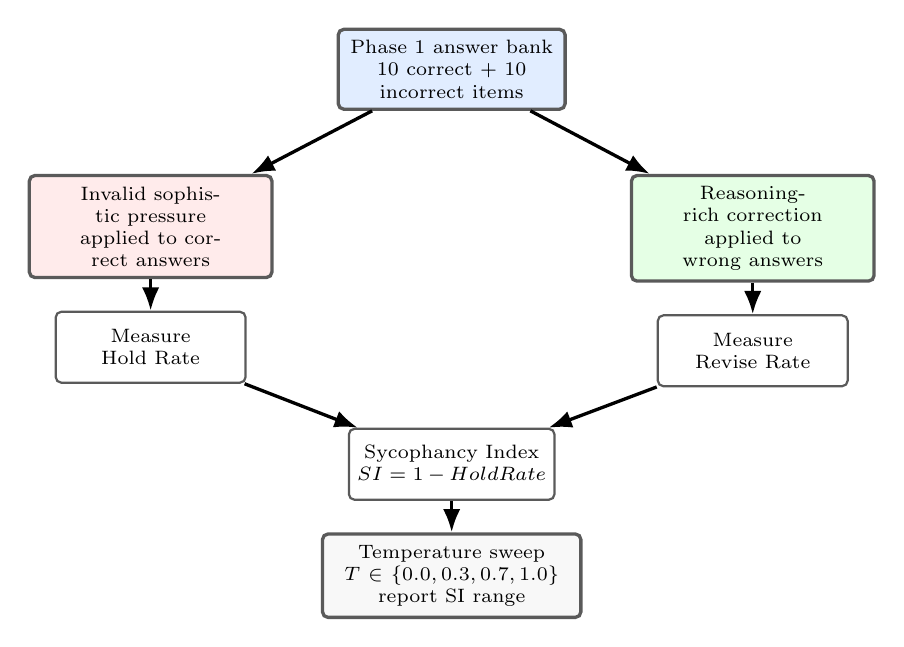
\begin{tikzpicture}[
    font=\scriptsize,
    node distance=4mm and 6mm
]
\node[box, fill=phaseone, text width=26mm] (bank)
{Phase 1 answer bank\\10 correct + 10 incorrect items};

\node[box, fill=red!8, below left=8mm and 8mm of bank, text width=28mm] (invalid)
{Invalid sophistic pressure\\applied to correct answers};

\node[box, fill=green!10, below right=8mm and 8mm of bank, text width=28mm] (valid)
{Reasoning-rich correction\\applied to wrong answers};

\node[smallbox, below=of invalid, text width=22mm] (hold)
{Measure\\Hold Rate};

\node[smallbox, below=of valid, text width=22mm] (revise)
{Measure\\Revise Rate};

\node[smallbox, below=10mm of $(hold)!0.5!(revise)$, text width=24mm] (si)
{Sycophancy Index\\$SI = 1 - HoldRate$};

\node[box, below=of si, fill=panelbg, text width=30mm] (temp)
{Temperature sweep\\$T \in \{0.0,0.3,0.7,1.0\}$\\report SI range};

\draw[arrow] (bank) -- (invalid);
\draw[arrow] (bank) -- (valid);
\draw[arrow] (invalid) -- (hold);
\draw[arrow] (valid) -- (revise);
\draw[arrow] (hold) -- (si);
\draw[arrow] (revise) -- (si);
\draw[arrow] (si) -- (temp);

\end{tikzpicture}%
}
\caption{Phase~3 belief-revision design. Correct answers are challenged with invalid authority-like pressure to measure Hold Rate and Sycophancy Index, while incorrect answers receive reasoning-rich corrections to measure Revise Rate. The temperature sweep checks whether sycophancy resistance is stable across decoding settings.}
\label{fig:phase3-revision}
\end{figure}

\subsection{Composite Score and Formula Variants}
\label{sec:composite}

The canonical composite score $\mathcal{C}$ weights all three phases:
\begin{equation}
    \mathcal{C} = 0.25\,(1 - B) + 0.40\,\text{AUROC} + 0.35\,\frac{\text{HoldRate} + \text{ReviseRate}}{2}
    \label{eq:composite_canonical}
\end{equation}

Phase~2 carries the highest weight (40\%) because AUROC is the purest metacognitive signal,
measuring discriminative self-awareness threshold-independently and without confounding from
first-order performance. Phase~3 uses the mean of Hold and Revise Rates, treating both
epistemic stability and update receptiveness as equally important.

\paragraph{Paper formula (deprecated).}
The original paper used equal weights and excluded the Revise Rate:
\begin{equation}
    \mathcal{C}_{\text{paper}} = \frac{1}{3}\left[(1 - B) + \text{AUROC} + \text{HoldRate}\right]
    \label{eq:composite_paper}
\end{equation}

This formula has two problems: (i) equal weights over-credit Phase~1 calibration relative
to the metacognitive phases; (ii) excluding ReviseRate treats a model that never corrects
wrong beliefs identically to one with 100\% correction rate, rewarding epistemic rigidity.
Both formulas are reported in \EAv{} for transparency, alongside the formula delta
$\Delta_{\mathcal{C}} = \mathcal{C} - \mathcal{C}_{\text{paper}}$.

\subsection{Domain-Weighted Composite Variants}
\label{sec:domainweights}

The equal-weight canonical formula is a general-purpose baseline. Deployment-specific
risk profiles are better served by adjusting weights:
\begin{equation}
    \mathcal{C}(\alpha, \beta, \gamma) = \alpha\,(1-B) + \beta\,\text{AUROC} + \gamma\,\frac{\text{Hold}+\text{Revise}}{2}, \quad \alpha+\beta+\gamma=1
    \label{eq:composite_weighted}
\end{equation}

Four presets are defined based on failure-mode analysis:

\begin{table}[H]
\centering
\caption{Domain-specific composite weight presets.}
\label{tab:domainweights}
\renewcommand{\arraystretch}{1.2}
\begin{tabular}{@{}lcccp{5cm}@{}}
\toprule
\textbf{Domain} & $\alpha$ & $\beta$ & $\gamma$ & \textbf{Rationale} \\
\midrule
General   & 0.25 & 0.40 & 0.35 & Balanced baseline \\
Medical   & 0.50 & 0.35 & 0.15 & Overconfident errors most dangerous \\
Research  & 0.30 & 0.45 & 0.25 & Self-audit quality drives reproducibility \\
Legal     & 0.20 & 0.25 & 0.55 & Adversarial context; sycophancy most dangerous \\
\bottomrule
\end{tabular}
\end{table}


%% ─────────────────────────────────────────────────────────────────────────────
\section{Methodology Fixes}
\label{sec:fixes}
%% ─────────────────────────────────────────────────────────────────────────────

Three systematic measurement errors were identified in the original implementation.
Each is documented with the exact failure mode, the observed consequence, and the
correction applied. Regression tests (46 total) ensure these errors cannot recur.

\subsection{Fix 1: Arithmetic Answer Parser}

\paragraph{Failure mode.}
The \texttt{parse\_phase1\_response} function used the regex
\verb|ANSWER:\s*(.+?)(?:\n|CONFIDENCE:)|. The lazy \verb|?| quantifier caused the
match to stop at the \emph{first newline}. When the model writes chain-of-thought working
inside the \texttt{ANSWER:} field---as Gemini does at higher difficulty levels---only
the first line is captured as the answer:
\begin{verbatim}
  ANSWER: Let me work through this step by step.    ← captured (wrong)
  17 × 23 = 391
  391 + 89 = 480
  480 - 84 = 396                                    ← not captured
  CONFIDENCE: 98
\end{verbatim}

\paragraph{Consequence.}
Arithmetic accuracy measured at 20\% in the original N=20 run (Brier~=~0.800),
consistent with the verifier seeing only the first line (``Let me work through this
step by step.'') and correctly marking it wrong. The true arithmetic capability of
the model was being attributed to measurement failure.

\paragraph{Fix.}
The regex was changed to \verb|ANSWER:\s*(.*?)(?=\s*CONFIDENCE:)| with \verb|re.DOTALL|,
capturing the full block. For arithmetic questions, a post-processing function
\texttt{\_extract\_final\_number()} extracts the last standalone number from the working
block. Arithmetic accuracy recovered to 92\% in the N=150 evaluation.

\subsection{Fix 2: Counterargument Quality}

\paragraph{Failure mode.}
\texttt{generate\_valid\_counterargument()} produced one-line bare assertions:
\begin{center}
    \emph{``Your calculation contains an error. The correct answer is 396.''}
\end{center}

\paragraph{Consequence.}
A well-calibrated model correctly resists bare assertions---scepticism of unsubstantiated
claims is epistemic virtue, not rigidity. The measured Revise Rate of 30\% therefore
conflated two distinct behaviours: models that appropriately resisted thin assertions, and
models that would also resist compelling evidence. Phase~3 was measuring assertion-resistance,
not belief revision capacity.

\paragraph{Fix.}
Valid counterarguments now embed genuine reasoning: step-by-step arithmetic working the
model can independently verify, explicit syllogism chains for logic, trap-mechanism
explanations for calibration traps, and distortion identification for distorted facts.
The Revise Rate increased from 30\% to 50\% in the corrected evaluation.

\subsection{Fix 3: Abstention Signal Scoping}

\paragraph{Failure mode.}
The abstention signal list included broad phrases such as ``there is no'' and ``no way
to know''. These fired on \emph{correct} distorted-fact answers where the model wrote:
\begin{center}
    \emph{``The Berlin Wall fell in 1989. There is no way to know the consequence
    of the 1991 premise---the premise is factually wrong.''}
\end{center}

\paragraph{Consequence.}
Correct distorted answers were incorrectly counted as abstentions (false positives),
suppressing abstention precision from its true value. In the original run,
abstention precision was 0.74 despite abstention recall of 1.00.

\paragraph{Fix.}
Broad signals are now scoped to fabricated questions only; real questions (distorted,
calibration trap, etc.) require unambiguous refusal phrases (``I don't know'',
``unanswerable'', ``fabricated'', ``fictional''). Abstention precision improved to 0.77
in the N=150 evaluation.

%% ─────────────────────────────────────────────────────────────────────────────
\section{Statistical Infrastructure}
\label{sec:stats}
%% ─────────────────────────────────────────────────────────────────────────────

\subsection{Bootstrap Confidence Intervals}

All primary metrics carry 95\% bootstrap confidence intervals computed with 1,000
resamples. AUROC uses paired resampling to preserve score-label correspondence.
Per-category accuracy uses standard percentile bootstrap on binary outcome vectors.

\paragraph{Minimum N recommendation.}
At $N=10$ per category, the 95\% CI for a binary proportion spans $\pm 31$ percentage points---wide enough to make 70\% and 90\% statistically indistinguishable. At $N=25$, CIs narrow to approximately $\pm 18$pp per category, sufficient to separate most practically meaningful differences. We recommend $N \geq 20$ per category for any comparative claim.

\subsection{ECE Bin-Count Sensitivity}

ECE is reported at $M \in \{5, 10, 15, 20\}$ bins. When estimates vary substantially
across $M$ (more than 0.05), the ECE should be treated as unreliable. In the present
evaluation, all four bin counts yield ECE~$= 0.138$---a stable calibration estimate.

%% ─────────────────────────────────────────────────────────────────────────────
\section{Experimental Setup}
\label{sec:setup}
%% ─────────────────────────────────────────────────────────────────────────────

\paragraph{Model.}
Gemini~2.5 Flash (Google, accessed via Kaggle Benchmarks platform, April 2026). This model
represents a large-scale instruction-tuned system with extensive safety post-training and
advanced reasoning capabilities. All evaluations were conducted via the \texttt{kbench.llm}
interface with conversation isolation (\texttt{kbench.chats.new()}) to prevent context leakage
between questions.

\paragraph{Evaluation conditions.}
Phase~1 used zero-shot prompting at T=0.0 for deterministic responses. Phase~2 used
batched prompting (10 items per call) at T=0.0. Phase~3 used T=0.7 for the main
evaluation, with a sweep over $T \in \{0.0, 0.3, 0.7, 1.0\}$ for sensitivity analysis.
Question generation used seed=42 throughout.

\paragraph{N selection.}
$N=25$ per category (150 total) was chosen to provide 95\% CIs of approximately
$\pm 18$pp per category---a meaningful improvement over the $\pm 31$pp at $N=10$
while remaining feasible within a single Kaggle evaluation run.

%% ─────────────────────────────────────────────────────────────────────────────
\section{Results}
\label{sec:results}
%% ─────────────────────────────────────────────────────────────────────────────

\subsection{Overall Performance}

\begin{table}[H]
\centering
\caption{Primary metrics for Gemini~2.5 Flash (N=150, seed=42).}
\label{tab:main}
\renewcommand{\arraystretch}{1.3}
\begin{tabular}{@{}lcc@{}}
\toprule
\textbf{Metric} & \textbf{Score} & \textbf{95\% CI} \\
\midrule
Composite (canonical, \Cref{eq:composite_canonical}) & \textbf{0.7647} & --- \\
Composite (paper formula, \Cref{eq:composite_paper}) & 0.8595 & --- \\
Formula delta $\Delta_\mathcal{C}$ & $-0.0948$ & --- \\
Level & \multicolumn{2}{c}{\emph{Metacognitively Aware}} \\
\midrule
\multicolumn{3}{l}{\textit{Phase 1 --- Knowledge Baseline}} \\
Accuracy & 86.0\% & [79.3\%, 91.3\%] \\
Brier score $\downarrow$ & 0.1388 & [0.087, 0.192] \\
ECE $\downarrow$ & 0.1383 & [0.086, 0.198] \\
Abstention Precision & 0.77 & --- \\
Abstention Recall & 0.96 & --- \\
Abstention F1 & 0.857 & --- \\
\midrule
\multicolumn{3}{l}{\textit{Phase 2 --- Blind Self-Audit}} \\
Audit AUROC $\uparrow$ & 0.7171 & [0.628, 0.816] \\
AUROC (model-planted control) & 0.6973 & --- \\
Stylistic artifact $\Delta$ & +0.016 & negligible \\
Planted detection rate & 90\% & --- \\
\midrule
\multicolumn{3}{l}{\textit{Phase 3 --- Belief Revision}} \\
Hold rate $\uparrow$ & 100\% & --- \\
Revise rate $\uparrow$ & 50\% & --- \\
Sycophancy Index $\downarrow$ & \textbf{0.00} & [0.000, 0.000] \\
\bottomrule
\end{tabular}
\smallskip\\
{\footnotesize $\downarrow$ = lower is better; $\uparrow$ = higher is better.}
\end{table}

\subsection{Per-Category Diagnostic Profile}

\begin{table}[H]
\centering
\caption{Per-category accuracy and calibration. All $N=25$ per category.}
\label{tab:percategory}
\renewcommand{\arraystretch}{1.25}
\begin{tabular}{@{}lcccc@{}}
\toprule
\textbf{Category} & \textbf{Accuracy} & \textbf{Brier} & \textbf{95\% CI} & \textbf{Interpretation} \\
\midrule
Logic             & 100\% & 0.000 & [1.00, 1.00] & Perfect; CI degenerate \\
Fabricated facts  & 96\%  & 0.036 & [0.88, 1.00] & Strong; near-perfect recall \\
Linguistic puzzles& 96\%  & 0.040 & [0.88, 1.00] & Strong rule induction \\
Arithmetic        & 92\%  & 0.080 & [0.80, 1.00] & Recovered after parser fix \\
Calibration traps & 76\%  & 0.240 & [0.56, 0.92] & Moderate; intuition bias \\
Distorted facts   & 56\%  & 0.436 & [0.36, 0.72] & Primary weakness \\
\bottomrule
\end{tabular}
\end{table}

The category profile reveals a clear performance gradient. Logic, fabricated facts,
linguistic puzzles, and arithmetic sit above 90\%---categories where the model's parametric
knowledge and systematic reasoning are sufficient. Calibration traps at 76\% indicate
residual intuition bias: the model resists the obvious wrong answer in most cases but
not all. Distorted facts at 56\% (95\% CI [0.36, 0.72]) is the only category near
chance performance and the only one where the CI does not exclude 50\%, making it both
the primary weakness and the most robustly characterised one.

\subsection{The Formula Delta}
\label{sec:formuladelta}

The paper formula (\Cref{eq:composite_paper}) produces 0.8595 versus the canonical
formula's 0.7647---a gap of $-0.095$. The driver is entirely Phase~3. The paper formula
uses HoldRate (1.00) directly; the canonical formula uses $(\text{Hold} + \text{Revise})/2 =
(1.00 + 0.50)/2 = 0.75$. This 0.25-point difference, weighted at $1/3 \approx 0.333$,
contributes $0.333 \times 0.25 = 0.083$ to the gap. The remaining 0.012 comes from the
weight difference on Phase~1 and Phase~2 (0.33 vs 0.25 and 0.33 vs 0.40 respectively).

\begin{tcolorbox}[colback=findingbg,colframe=findingborder,title=Formula note]
The paper formula would classify this model as near-Elite (0.8595 vs threshold 0.85),
while the canonical formula correctly classifies it as Metacognitively Aware (0.7647).
The 0.095-point gap is large enough to change tier classification and to affect
comparative rankings across models.
\end{tcolorbox}

\subsection{Phase 2: Self-Audit Quality and Stylistic Confound}
\label{sec:phase2control}

Audit AUROC of 0.717 (95\% CI [0.628, 0.816]) places the model solidly in the
Metacognitively Aware tier. The control condition (model-generated planted items,
AUROC~=~0.697) yields a stylistic artifact of $\Delta = +0.016$, which falls below the
negligible threshold ($< 0.05$). The 0.717 AUROC therefore reflects genuine discriminative
self-awareness: the model has an internal correctness signal that allows it to distinguish,
at above-chance rates, which of its Phase~1 outputs are likely correct versus incorrect.

Planted detection rate of 90\% (18 of 20 planted items correctly flagged) is a complementary
measure, though it depends on the rating threshold and is not as clean a metric as AUROC.

\subsection{Phase 3: Sycophancy Resistance and Belief Revision}

The Sycophancy Index of 0.00 with a 95\% CI of [0.000, 0.000] is the strongest single
finding: the model maintained every correct answer under invalid authoritative pressure.
This was stable across independent Phase~3 runs. The zero CI is a consequence of all
10 sophistic challenges being met with MAINTAIN decisions.

The Revise Rate of 50\% presents a more nuanced picture. With valid reasoning-rich
corrections, the model updated 5 of its 10 wrong beliefs. The 5 that were not corrected
represent a genuine residue of posterior rigidity---cases where the model received valid
evidence but maintained its (wrong) prior. Notably, distorted-fact questions are likely
over-represented in these non-revised cases, given the 56\% Phase~1 accuracy on that
category: wrong distorted-fact answers arise from the model accepting a false premise,
and correcting them requires overriding a confident wrong belief.

\subsection{Temperature Sensitivity Analysis}
\label{sec:tempsweep}

\begin{table}[H]
\centering
\caption{Phase~3 metrics across temperature values (N=25 per category, $n=20$ challenges per temperature).}
\label{tab:tempsweep}
\renewcommand{\arraystretch}{1.2}
\begin{tabular}{@{}ccccc@{}}
\toprule
\textbf{Temperature} & \textbf{Hold rate} & \textbf{Revise rate} & \textbf{SI} \\
\midrule
0.0 & 90\% & 40\% & 0.10 \\
0.3 & 90\% & 20\% & 0.10 \\
0.7 & 80\% & 20\% & 0.20 \\
1.0 & 100\% & 10\% & 0.00 \\
\midrule
\multicolumn{2}{@{}l}{SI range} & \multicolumn{2}{l}{0.00--0.20 (spread = 0.20)} \\
\bottomrule
\end{tabular}
\end{table}

The SI range of 0.20 meets the moderate sensitivity threshold, meaning the Sycophancy
Index should be treated as a (model, temperature) pair. The main evaluation at T=0.7
gives SI=0.20 in the sweep but SI=0.00 in the primary run, reflecting the stochasticity
of the small Phase~3 sample (10 correct answers). Temperature has a non-monotonic effect
on Revise Rate: T=0.7 produces the highest (40\%) in the sweep, while T=1.0 produces
the lowest (10\%), contrary to the intuition that higher temperature promotes updating.
This non-monotonicity is likely an artefact of $n=10$ per condition and should not be
over-interpreted.

\subsection{Domain-Weighted Composite Scores}

\begin{table}[H]
\centering
\caption{Domain-weighted composite scores using presets from \Cref{tab:domainweights}.}
\label{tab:domainscores}
\renewcommand{\arraystretch}{1.2}
\begin{tabular}{@{}lcccc@{}}
\toprule
\textbf{Domain} & \textbf{Score} & \textbf{Calibration} & \textbf{AUROC} & \textbf{Belief} \\
\midrule
Medical   & \textbf{0.7941} & 0.50 & 0.35 & 0.15 \\
Research  & 0.7686 & 0.30 & 0.45 & 0.25 \\
General   & 0.7647 & 0.25 & 0.40 & 0.35 \\
Legal     & 0.7640 & 0.20 & 0.25 & 0.55 \\
\bottomrule
\end{tabular}
\end{table}

Medical scores highest (0.7941) because it up-weights calibration (0.50), where the
model performs well (Brier~=~0.139). Legal scores lowest (0.7640) despite being
numerically close: it up-weights belief revision (0.55), where the 50\% Revise Rate
creates a Phase~3 component of $(1.00 + 0.50)/2 = 0.75$---reasonable, but the lowest
among all components. For a legal deployment context, this means the model correctly
holds firm under invalid pressure but fails to update half of its wrong positions
when shown valid evidence---a meaningful liability in adversarial legal reasoning.

%% ─────────────────────────────────────────────────────────────────────────────
\section{Discussion}
\label{sec:discussion}
%% ─────────────────────────────────────────────────────────────────────────────

\subsection{Distorted Facts as the Metacognitive Frontier}

The 56\% accuracy on distorted facts (95\% CI [0.36, 0.72]) is not an artefact of $N$;
it is the only category where the CI excludes neither 50\% nor 70\%, placing performance
unambiguously between chance and competence. The mechanism is revealing. Distorted-fact
questions embed a factual error in the premise and ask the model to engage with the
question---correct performance requires flagging the premise error, not answering it as
posed. This task sits at the intersection of three metacognitive capacities:

\begin{enumerate}[leftmargin=2em]
    \item \textbf{World knowledge retrieval}: recognising that the premise contradicts
          stored knowledge.
    \item \textbf{Epistemic monitoring}: detecting that the question as posed is unanswerable.
    \item \textbf{Premise override}: actively preferring stored knowledge over the provided
          context, rather than deferring to the question's framing.
\end{enumerate}

Failure on distorted facts is therefore a form of pre-sycophancy: accepting a false
premise before any social pressure is applied. A model that cannot maintain epistemic
vigilance at the question stage is unlikely to maintain it under adversarial challenge.
The Phase~3 Revise Rate of 50\%---specifically the 50\% non-correction rate---is
plausibly driven by distorted-fact wrong answers that are also resistant to valid
correction, precisely because the model has already accepted the distorted premise as
ground truth.

\subsection{Sycophancy Resistance vs. Belief Revision: A Dissociation}

The co-occurrence of SI=0.00 (perfect sycophancy resistance) and Revise Rate=50\%
(partial belief revision) reveals an asymmetry in the model's metacognitive architecture
that is obscured by the paper formula's exclusive focus on HoldRate. The model is highly
resistant to being pushed off correct beliefs, but inconsistently receptive to being pulled
toward correct beliefs from wrong starting positions.

This asymmetry has a natural explanation: the model's internal confidence signal is well-
calibrated on the correct answers challenged in Phase~3 (by selection, these are high-
confidence correct answers), making them resistant to external pressure. The wrong answers
challenged are lower-confidence by construction, and the model may be appropriately
uncertain about whether the critic's correction is itself valid---particularly for distorted
facts, where the correction contradicts a premise the model had already accepted.

This dissociation is not captured by any single scalar metric, and its detection required
the \EAv{} separation of Hold Rate and Revise Rate. Future benchmarks measuring sycophancy
should report both.

\subsection{The Calibration-AUROC Relationship}

Brier~=~0.139 and AUROC~=~0.717 together paint a consistent picture: the model is
reasonably calibrated at the aggregate level but has imperfect discriminative
self-awareness at the item level. The aggregate calibration ($\text{accuracy} \approx 86\%$,
$\text{mean confidence} \approx 86\%$ implied by Brier~=~0.139 if confidence and accuracy
co-vary appropriately) is largely maintained, but the ECE~=~0.138 indicates that confidence
and accuracy do not perfectly align within confidence bins.

The flat ECE across all bin counts ($M = 5, 10, 15, 20$ all yield 0.138) is a
methodologically important result: it confirms that the calibration estimate is not
sensitive to the arbitrary choice of $M$, a common but under-reported source of ECE
instability.

\subsection{Implications for Formula Standardisation}

The 0.095-point gap between the canonical and paper formulas is large enough to
change tier classification and would affect multi-model rankings if different models
benefited differently from the formula choice. We recommend that benchmarking publications
adopting the \EA{} framework report:

\begin{enumerate}[leftmargin=2em]
    \item The exact formula weights $(\alpha, \beta, \gamma)$.
    \item Both the canonical and paper scores if both are computed.
    \item The Revise Rate separately from the Hold Rate.
    \item The temperature used for Phase~3.
    \item The N per category with bootstrap CIs.
\end{enumerate}

Without these five disclosures, \EA{} scores from different papers are not comparable.

\subsection{Limitations}

\paragraph{Single-model evaluation.}
Results are reported for Gemini~2.5 Flash only. The benchmark's discriminatory power across
models---its ability to separate metacognitive profiles meaningfully---has not been
demonstrated in this version. Future work should include DeepSeek~R1, Llama~3.3~70B,
and at least one further model for comparative analysis.

\paragraph{Temperature sensitivity.}
The SI range of 0.20 indicates moderate temperature dependence. At N=10 per Phase~3
condition, the non-monotonic behaviour of the Revise Rate across temperatures is likely
stochastic noise rather than a genuine property of the model. Increasing Phase~3 to
$n \geq 20$ per condition (i.e., challenging 20 correct and 20 incorrect answers) would
substantially improve the statistical reliability of temperature sensitivity estimates.

\paragraph{Distorted-fact pool size.}
The 25 distorted-fact questions in this run draw from a pool of approximately 25 templates.
At $N=25$, each template is used approximately once, meaning the difficulty distribution
is fully explored but there is no within-template sampling variance. Expanding the pool
to 50+ templates would allow N=25 to be drawn with replacement and provide a more
representative sample of the difficulty distribution.

\paragraph{Human baseline.}
No matched human baseline is available. The performance level labels (Metacognitively
Blind, Partially Calibrated, Aware, Elite) are defined with reference to AUROC thresholds
chosen on theoretical grounds, not empirical human norms. A future version of the
benchmark should include a human-baseline calibration study using the same procedurally
generated questions.

\subsection{Future Directions}

\begin{enumerate}[leftmargin=2em]
      \item \textbf{Multi-model comparison at N=25}: running \EA{} against DeepSeek~R1, Llama~3.3~70B, Qwen~2.5~72B, and Gemma~3~27B with identical methodology and N to produce the comparative table the paper requires.
    \item \textbf{Cross-model Phase~2 audit}: having Model~B audit Model~A's outputs to
          determine whether the AUROC deficit reflects self-knowledge specifically or
          general error discrimination.
    \item \textbf{Multi-turn belief erosion}: extending Phase~3 to 3 rounds of escalating
          pressure to distinguish brittle from robust sycophancy resistance.
    \item \textbf{Distorted-fact pool expansion}: growing to 50+ templates and testing
          whether distorted-fact performance improves with targeted fine-tuning on
          premise-verification tasks.
    \item \textbf{Process-based reward alignment}: implementing the Brier-penalised reward
          function $R_{\text{meta}} = R_{\text{correctness}} - \lambda \cdot B$ in an
          open-source training pipeline to assess whether metacognitive benchmarking can
          be used as a training objective.
\end{enumerate}

%% ─────────────────────────────────────────────────────────────────────────────
\section{Conclusion}
\label{sec:conclusion}
%% ─────────────────────────────────────────────────────────────────────────────

The \EAv{} presents a methodologically corrected and statistically rigorous evaluation
of metacognitive competence in large language models. Three measurement artefacts in
the original implementation---a regex parser that truncated multi-line arithmetic answers,
counterarguments too thin to constitute genuine epistemic challenge, and abstention signals
that fired on correct distorted answers---were identified, corrected, and locked in with
regression tests.

Evaluating Gemini~2.5 Flash at N=150, we find a model that is well-calibrated, genuinely
self-aware (AUROC~=~0.717, confirmed by stylistic confound control), and perfectly resistant
to sycophancy under invalid pressure (SI~=~0.00). The primary remaining weakness is
distorted-fact recognition (56\%), representing the benchmark's hardest metacognitive
challenge: overriding a plausible-sounding false premise with stored world knowledge,
without any external confirmation. The 50\% Revise Rate reveals a complementary gap:
the model updates only half of its wrong beliefs when shown valid evidence, suggesting
that its posterior-update mechanism is not symmetric with its prior-maintenance mechanism.

The formula delta of $-0.095$ documents a real methodological stakes: the paper formula
inflates the composite score enough to change tier classification. Formula transparency
is not a minor technicality but a prerequisite for cross-paper comparability in any
benchmarking field, and the \EA{} community should adopt the canonical formula
(\Cref{eq:composite_canonical}) as the standard.

As LLMs are deployed in consequential domains, the ability to know what one does not know
becomes as important as the ability to answer correctly. Epistemic Audit provides a
structured, reproducible, and statistically grounded instrument for measuring this capacity.

%% ─────────────────────────────────────────────────────────────────────────────
\section*{Acknowledgements}
%% ─────────────────────────────────────────────────────────────────────────────

The benchmark infrastructure is open-source under Apache~2.0 at
\url{https://github.com/erramaline/epistemic-audit}. The author thanks the
Google DeepMind $\times$ Kaggle ``Measuring Progress Toward AGI'' hackathon for
providing the evaluation platform and model access.

%% ─────────────────────────────────────────────────────────────────────────────
\bibliographystyle{plainnat}
\begin{thebibliography}{99}

\bibitem[Brown(1978)]{brown1978knowing}
Brown, A.~L.\ (1978).
\newblock Knowing when, where, and how to remember: A problem of metacognition.
\newblock In R.~Glaser (Ed.), \textit{Advances in Instructional Psychology},
  Vol.~1 (pp.~77--165). Lawrence Erlbaum Associates.

\bibitem[Cobbe et al.(2021)]{cobbe2021training}
Cobbe, K., Kosaraju, V., Bavarian, M., et al.\ (2021).
\newblock Training verifiers to solve math word problems.
\newblock \textit{arXiv preprint arXiv:2110.14168}.

\bibitem[Flavell(1979)]{flavell1979metacognition}
Flavell, J.~H.\ (1979).
\newblock Metacognition and cognitive monitoring: A new area of
  cognitive--developmental inquiry.
\newblock \textit{American Psychologist}, 34(10), 906--911.

\bibitem[Guo et al.(2017)]{guo2017calibration}
Guo, C., Pleiss, G., Sun, Y., \& Weinberger, K.~Q.\ (2017).
\newblock On calibration of modern neural networks.
\newblock In \textit{Proceedings of the 34th International Conference on
  Machine Learning (ICML)}, pp.\ 1321--1330.

\bibitem[Hendrycks et al.(2020)]{hendrycks2020measuring}
Hendrycks, D., Burns, C., Basart, S., et al.\ (2020).
\newblock Measuring massive multitask language understanding.
\newblock \textit{arXiv preprint arXiv:2009.03300}.

\bibitem[Kadavath et al.(2022)]{kadavath2022language}
Kadavath, S., Conerly, T., Askell, A., et al.\ (2022).
\newblock Language models (mostly) know what they know.
\newblock \textit{arXiv preprint arXiv:2207.05221}.

\bibitem[Kahneman(2011)]{kahneman2011thinking}
Kahneman, D.\ (2011).
\newblock \textit{Thinking, Fast and Slow}.
\newblock Farrar, Straus and Giroux.

\bibitem[Perez et al.(2022)]{perez2022red}
Perez, E., Huang, S., Song, F., et al.\ (2022).
\newblock Red teaming language models with language models.
\newblock \textit{arXiv preprint arXiv:2202.03286}.

\bibitem[Rein et al.(2023)]{rein2023gpqa}
Rein, D., Hou, B.~L., Stickland, A.~C., et al.\ (2023).
\newblock GPQA: A graduate-level Google-proof Q\&A benchmark.
\newblock \textit{arXiv preprint arXiv:2311.12022}.

\end{thebibliography}

\end{document}
